% Nallino, Part II p. 243, second figure: the equations of Mercury, redrawn from the print at the size of the print.
% The coordinates are those of a 400 dpi render of the figure (crop from x 322 pt, y 425 pt of the master page;
% y downward). The arc YZX belongs to the ecliptic about the Earth E; GK is the line of apsides of the equant;
% the circellus has its centre in F, the centre M of the deferent and the centre E' of the equant on it; the epicycle
% has its centre in H, the planet in T, the true apogee P and the mean apogee Q. Dashed as on the print: HM, MI, IE',
% E'N and NE. The double arcs mark the equal angles GFI and GE'H. A stray dot to the right of GK is not drawn.
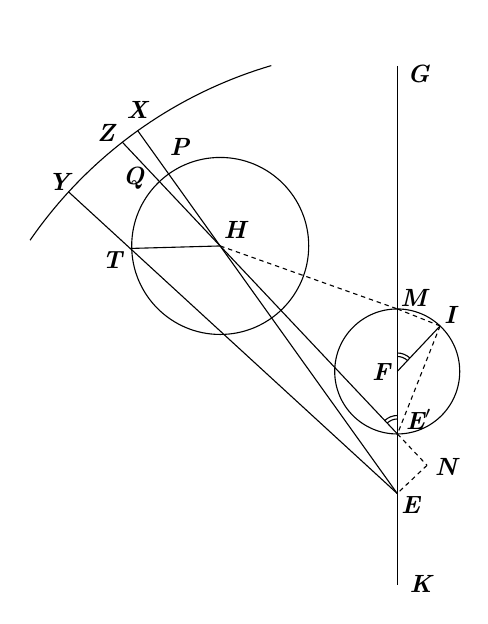
\begin{tikzpicture}[x=0.0635mm,y=-0.0635mm,line width=0.4pt,every node/.style={font=\bfseries\itshape\small,inner sep=1pt}]
\path (40,38.5);
\coordinate (E) at (779,970);
\coordinate (Ep) at (779.5,851);
\coordinate (M) at (779.5,601);
\coordinate (F) at (779,726);
\coordinate (I) at (864.7,635);
\coordinate (N) at (838.6,913.7);
\coordinate (H) at (425,475);
\coordinate (T) at (245,480);
\coordinate (X) at (260,244.4);
\coordinate (Z) at (229.3,267.5);
\coordinate (Y) at (121.8,366.9);
\draw (E) ++(214.6:892) arc[start angle=214.6, end angle=253.6, radius=892];
\draw (779.5,115) -- (779.5,1153);
\draw (H) circle[radius=177];
\draw (F) circle[radius=125];
\draw (E) -- (X);
\draw (Ep) -- (Z);
\draw (E) -- (Y);
\draw (H) -- (T);
\draw (F) -- (I);
\begin{scope}[dash pattern=on 1.6pt off 1.4pt]
\draw (H) -- (M);
\draw (M) -- (I);
\draw (I) -- (Ep);
\draw (Ep) -- (N);
\draw (N) -- (E);
\end{scope}
\draw (F) ++(-90:30) arc[start angle=-90, end angle=-47, radius=30];
\draw (F) ++(-90:37) arc[start angle=-90, end angle=-47, radius=37];
\draw (Ep) ++(-90:30) arc[start angle=-90, end angle=-133.3, radius=30];
\draw (Ep) ++(-90:37) arc[start angle=-90, end angle=-133.3, radius=37];
\node at (821.5,130.5) {G};
\node at (259,203.5) {X};
\node at (196.5,250) {Z};
\node at (343.5,277) {P};
\node at (251.5,339.5) {Q};
\node at (102.5,347) {Y};
\node at (454,442.5) {H};
\node at (209,502.5) {T};
\node at (812,580) {M};
\node at (884.5,613) {I};
\node at (747,726.5) {F};
\node at (815,822) {E\rlap{$'$}};
\node at (876.5,917) {N};
\node at (805.5,992) {E};
\node at (826,1151.5) {K};
\end{tikzpicture}
